%!TEX root=./paper.tex
\subsection{\textbf{Model input}}

For each node, a composite feature vector is constructed to encapsulate all pertinent node-related data. This vector is formed by concatenating three distinct feature vectors, each defined as follows:

\subsubsection{Graph embedding generation using Node2Vec:}\label{subsubsec:embd}

To facilitate the model's understanding of spatial relationships among detector nodes within the graph structure, an effective representation of the nodes' neighborhood structure is essential. Node2Vec \cite{node2vec} addresses this need through a feature learning approach that employs second-order biased random walks within a Skip-gram architecture. The process of generating feature vectors involves two pivotal steps:


\begin{enumerate}[(i)]
    \item \textit{Sampling using second-order biased random walks}: Two hyper-parameters, \( p \) and \( q \), are introduced in the context of Node2Vec, where \( p \) controls the likelihood of revisiting nodes in the random walk (termed as the "return" parameter), and \( q \) adjusts the likelihood of exploring nodes further away from the current node (termed as the "in-out" parameter). Let \( l \) denote the fixed length of the simulated random walk starting at node \( u \), with \( c_i \) representing the \( i \)th node in the walk (\( c_0 = u \)). Nodes \( c_i \) are generated according to the following distribution:

    \[
        P(c_i = x \mid c_{i-1} = v) =
        \begin{cases}
        \frac{\pi_{vx}}{Z} & \text{if } (v,x) \in E \\
        0 & \text{otherwise}
        \end{cases}
    \]
    where \( \pi_{vx} \) is the unnormalized transition probability between nodes \( v \) and \( x \), and \( Z \) is the normalizing constant.
    
    For a random walk that has just traversed edge \( (t,v) \) and is currently at node \( v \), the next step involves evaluating transition probabilities \( \pi_{vx} \) for edges \( (v,x) \) leading from \( v \). Here, the transition probability is determined by \( \pi_{vx} = \alpha_{pq}(t,x) \cdot w_{vx} \), where \( \alpha_{pq}(t,x) \) denotes the transition probability adjustment factor defined as:

    \[
        \alpha_{pq}(t,x) = 
        \begin{cases}
        \frac{1}{p}  & \text{if } d_{tx} = 0\\
        1 & \text{if } d_{tx} = 1\\
        \frac{1}{q} & \text{if } d_{tx} = 2
        \end{cases}
    \]
    and \( d_{tx} \) denotes the shortest path distance between nodes \( t \) and \( x \).

    \item \textit{Optimizing objective function using Skip-gram}: Let \( G(V, E) \) be a graph where \( f: V \rightarrow \mathbb{R}^d \) denotes the function mapping each node \( u \) to a \( d \)-dimensional feature representation. Hence, \( f \) forms a matrix of parameters sized \( |V| \times d \). For each node \( u \in V \), let \( N_S(u) \subset V \) represent the \emph{network neighborhood} generated in step (i). The similarity between nodes \( u \) and \( v \) is defined as:

    \[
        P_f(v|u) = \frac{\exp(f(v)^T f(u))}{\sum_{w \in V} \exp(f(w)^T f(u))} \tag{1}
    \]
    For neighborhood \( N_s(v) \) of \( v \), define the probability of the neighborhood of \( u \) as:
    
    \[ P_f(N_s(u)|u) = \prod_{v \in N_s(u)} P_f(v|u) \tag{2} \]

    Further, the global neighborhood likelihood for a given \( f \) can be defined as:
\[ \sum_{u \in V} \log P_f(N_s(u) \mid u) \tag{3} \]
which is the objective function that we want to maximize through the feature representation function \(f\). Hence,
\[ \max_{u \in V} \sum_{u \in V} \log \left( \prod_{v \in N_s(u)} \frac{\exp(f(v)^T f(u))}{\sum_{w \in V} \exp(f(w)^T f(u))} \right) \tag{4} \]

\end{enumerate}

\begin{figure*}[htbp]
  \centering
  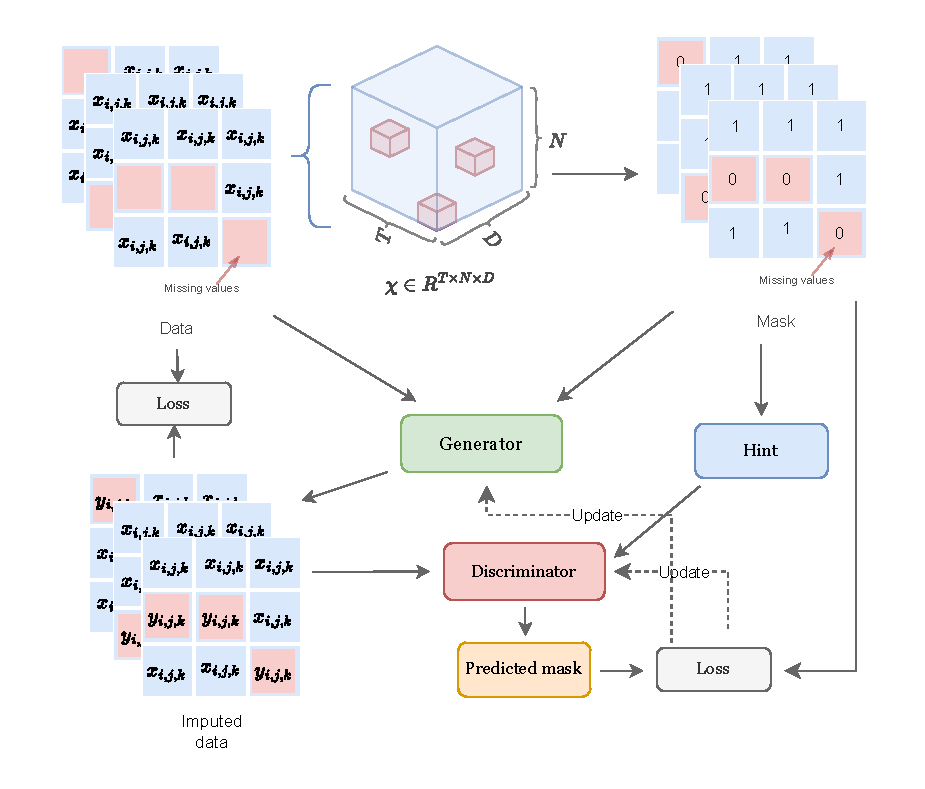
\includegraphics[width=0.85\textwidth]{model.pdf}
  \caption{\name \ architecture}
  \label{fig:architecture}
\end{figure*}

\subsubsection{Normalizing traffic volume}\label{subsubsec:normal}
The input data should be normalized to increase the training speed and effectiveness. The traffic volume counts at different detectors are normalized as follows:

\[ x_{\text{norm}} = \frac{x - x_{\text{min}}}{x_{\text{max}} - x_{\text{min}}} \]
Thus, \( x_{\text{norm}} \) is in the range \([0,1]\) after normalization.
This same approach is used for other continuous or discrete single-valued features.

\subsubsection{Word2Vec encoding of other exogenous variables:}\label{subsubsec:encode}
The Skip-gram architecture, a prominent model in natural language processing~\cite{skipgram}, operates under the Word2Vec framework~\cite{word2vec}. Its primary objective is to predict surrounding context words based on a given target word. By doing so, Skip-gram effectively learns to encode semantic meanings of words by maximizing the conditional probability of context words given the target word. This objective function is mathematically formulated as:
\[
J_\theta = \frac{1}{T}\sum^{T}_{t=1}\sum_{-n\leq j \leq n, j \neq 0}\log p\left(w_{j+1} \mid w_{t}\right)
\]

where \( w_t \) represents the target word at position \( t \), \( c \) is the size of the context window, and \( T \) is the total number of words in the corpus.

In our methodology, we employ \textit{Word2Vec} \cite{word2vec} to encode various exogenous variables such as weather conditions, road types, and other potentially relevant factors into feature vectors for the model input. This enhancement aims to augment the model's effectiveness by capturing semantic relationships between these variables and the observed traffic patterns. Importantly, our approach is designed to accommodate future extensions, allowing for the inclusion of additional relevant features as they are identified and integrated into the model input.

Concatenating the feature vectors obtained from Sections~\ref{subsubsec:embd} to \ref{subsubsec:encode}, we derive the final input vector for our model. Extending upon the notation introduced in Section~\ref{sec:problem-for}, for $N$ nodes, we define $\mathbf{x}_i^t$, the feature vector of node $i$ at time $t$. Assuming the use of \textit{Node2Vec} as described in (i) to generate $R^{D_g}$-dimensional graph embeddings $g_i$ for each node $i$, and normalizing $n$ single-dimensional real-valued features $(r_1, r_2, \ldots, r_n)$ as outlined in (ii) to $(r_1^{\text{norm}}, r_2^{\text{norm}}, \ldots, r_n^{\text{norm}})$, resulting in a $D_n = n$ dimensional vector $h_i^t$. Additionally, leveraging \textit{Word2Vec} to produce $d_w$ dimensional vectors for $m$ semantic "words" related to each node, we obtain a $R^{m \times d_w}$-dimensional vector flattened and represented as $k_i^t \in R^{D_w}$, where $D_w = m \times d_w$.

Finally, by concatenating the feature vectors described in Section~\ref{subsubsec:embd} -~\ref{subsubsec:encode}, we obtain the feature vector of node $i$ at time $t$:
\[
\mathbf{x}_i^t = ( g_i || h_i^t || k_i^t ) \in \mathbb{R}^D
\]
where $D = D_g + D_n + D_w$. Thus, leveraging the methodologies outlined in Eq~(\ref{eq:X}) and (\ref{eq:chi}), across $T$ consecutive time steps and for $N$ nodes, we construct the final feature vector $\mathbf{\chi} \in \mathbb{R}^{T \times N \times D}$. Depending on the specific task, additional inputs such as a binary matrix $M$ representing missing and known values are included. %Further implementation details are discussed in the experiments section.
